%\documentclass[xetex,mathserif,serif]{beamer}
\documentclass{beamer}
\renewcommand{\tiny}{\fontsize{4}{14}\selectfont}

\usepackage{hyperref}
\usepackage{fontspec} 
\usepackage{xunicode} %Unicode extras!
\usepackage{xltxtra} %Fixes 
\usefonttheme{professionalfonts}
\setmainfont{Linux Libertine}
%\setmonofont[Scale=0.86]{DejaVu Sans Mono}
\setmonofont{Liberation Mono}
%\setromanfont{Silkscreen}
%\setsansfont{DejaVu Sans}
\setsansfont{Droid Sans}

\usepackage[final,expansion=true,protrusion=true,spacing=true,kerning=true]{microtype}
\usetheme{openlab} 
\setbeamertemplate{navigation symbols}{}
\usepackage{graphicx}

\title[Developers]{Open IT Lab} 
\author{Jarrell Waggoner} 
\institute[Open IT Lab] {Open IT Lab\\
  \medskip
      {\emph{waggonej@email.sc.edu}} }
\date{\today}

\usebackgroundtemplate{
\includegraphics[width=\paperwidth]{../img/bg.png}}

% Videos/websites to show:
% About SFD: http://softwarefreedomday.org/
% Dictionary Definition: http://dictionary.reference.com/browse/open
% RSA Animate: http://youtu.be/u6XAPnuFjJc?t=6m44s
% Karen Sandler: http://youtu.be/nFZGpES-St8?t=2m26s
% My video
% Thing-O-Matic Video: http://www.flickr.com/photos/retrocactus/6044172663/
% Arduino projects: http://hacknmod.com/hack/top-40-arduino-projects-of-the-web/
% Free Content: http://questioncopyright.org/understanding_free_content
% Open Cola Ingredients: http://en.wikipedia.org/wiki/OpenCola_%28drink%29
% Creative Commons Selection: http://creativecommons.org/choose/

\begin{document}
\rm

% {
%   \usebackgroundtemplate{
\includegraphics[width=\paperwidth]{../img/bg-title.png}} 
%   \begin{frame}
% %    \titlepage
%     \vspace{18em}

%     \begin{center}\large{\textcolor{beamer@mygrey}{Jarrell Waggoner}}\end{center}

% %    \begin{center}\small{\textcolor{beamer@mygreen}{waggonej@email.sc.edu}}\end{center}

% %    \begin{center}\small{\textcolor{beamer@mygrey}{\today}}\end{center}
%   \end{frame}
% }

\begin{frame}
  \frametitle{Introduction}
  % \begin{center}\begin{LARGE}Open Source: The Great Equalizer\end{LARGE}\end{center}
  \begin{center}
    
\includegraphics[width=0.25\textwidth]{../img/tux-rambo}   

    \vspace{2em}

    \begin{Huge}Open Source:\end{Huge} \\ \begin{LARGE}How Do You Get Involved\end{LARGE}
  \end{center}
\end{frame}

% \begin{frame}
%   \frametitle{About Me}
%   \begin{LARGE}
%     Jarrell Waggoner
%   \end{LARGE}
%   \begin{Large}
%     \begin{itemize}
%     \item Ph.D. candidate in computer science at the College of
%       Engineering and Computing at USC
%     \item Been writing software for 15 years
%     \item Using open source and creating open content since 1998
%     \item Created an open movie in 2006
%     \item Teaching programming and software development using open source tools since 2007
%     \item Website: \textcolor{beamer@myblue}{\href{http://www.malloc47.com}{http://www.malloc47.com}}
%     \end{itemize}
%   \end{Large}
% \end{frame}

\begin{frame}
  \frametitle{How?}
  \begin{itemize}
    \setlength{\itemsep}{2em}
  \item \begin{LARGE} \textcolor<2>{beamer@myblue}{Contribute} \end{LARGE} \\ \textcolor<2>{beamer@myblue}{(to existing projects)} \\
  \item \begin{LARGE} \textcolor<2>{beamer@mygrey}{Create} \end{LARGE} \\ \textcolor<2>{beamer@mygrey}{(your own projects and make them open source)}
  \end{itemize}
\end{frame}

\begin{frame}
  \frametitle{What can you contribute?}
  \begin{columns}[c]
    \column{0.4\textwidth}
    \begin{itemize}
    \item \textcolor<2>{beamer@mygrey}{Testing/Bug reports}
    \item \textcolor<2>{beamer@mygrey}{Writing/Documentation}
    \item \textcolor<2>{beamer@mygrey}{Support}
    \item \textcolor<2>{beamer@mygrey}{Tutorials}
    \item \textcolor<2>{beamer@mygrey}{Start a group}
    \item \textcolor<2>{beamer@mygrey}{Share}
    \item \textcolor<2>{beamer@mygrey}{Remix}
    \item \textcolor<2>{beamer@mygrey}{Graphics/Design}
    \item \textcolor<2>{beamer@myblue}{Programming}
    \end{itemize}
    \column{0.55\textwidth}
    
\includegraphics[width=1\textwidth]{../img/tux-question-3}
  \end{columns}
\end{frame}

\begin{frame}
  \frametitle{Where to look}
  \begin{columns}[c]
    \column{0.5\textwidth}
    \begin{itemize}
    \item openhatch.org
    \item Software communities 
      \begin{itemize}
      \item github
      \item Bitbucket
      \item Google Code
      \item SourceForge
      \end{itemize}
    \item Hardware communities
      \begin{itemize}
      \item openhardwarehub.com
      \item opendesignengine.net
      \end{itemize}
      % http://www.slideshare.net/kfasimpaur/open-educational-resources-share-remix-learn-v4
    \item Content communities
      \begin{itemize}
      \item Wikimedia Commons
      \item Open Photo Project
      % \item musopen
      % \item ccMixter
      \item KahnAcademy
      \item Curriki
      \item OER Commons
      \end{itemize}
    \item Whatever you're already using!
    \end{itemize}
    \column{0.45\textwidth}
    
\includegraphics[width=1\textwidth]{../img/carmen-sandiego}
  \end{columns}
\end{frame}

\begin{frame}
  \frametitle{Who to go to?}
  \begin{columns}[c]
    \column{0.6\textwidth}
    \begin{description}
    \item[Maintainers] who manage the project you're interested in
    \item[Websites] for the project may have a "get involved" section
    \item[Professors] may let you make your projects open source and guide you in getting involved
    \item[Employers] Open Source team experience \textbf{IS} 21st century employment
    \end{description}
    \column{0.4\textwidth}
    
\includegraphics[width=0.8\textwidth]{../img/dr-who}
  \end{columns}
\end{frame}

\begin{frame}
  \frametitle{Mozilla}
  \begin{center} 
    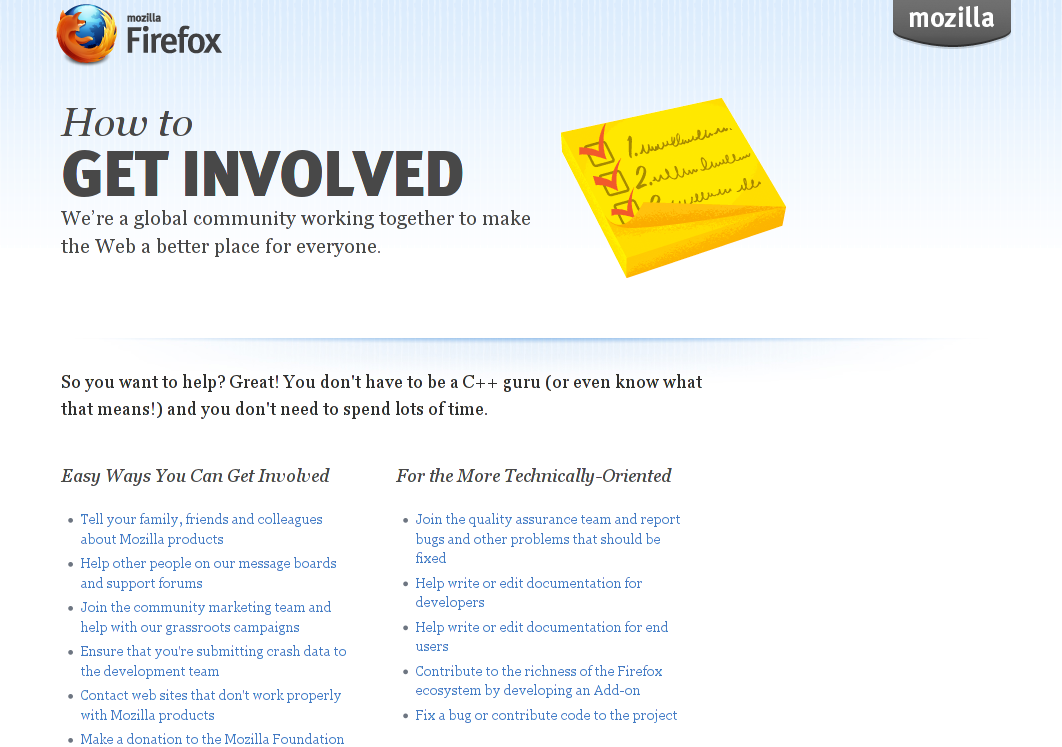
\includegraphics[height=0.8\textheight]{../img/mozilla-get-involved}

    \href{http://www.mozilla.org/en-US/firefox/community/}{http://www.mozilla.org/en-US/firefox/community/}
  \end{center}
\end{frame}

\begin{frame}
  \begin{columns}[c]
    \column{0.6\textwidth}
    \frametitle{How do you get paid?}
    \begin{itemize}
    \item Summer-of-Codes
      \begin{itemize}
      \item Google SOC
      \item Ruby SOC
      \item New Zealand SOC
      \end{itemize}
    \item Internships at OS-friendly companies \\ (Red Hat, Mozilla,
      Untangle, Canonical, etc.)
      % http://www.networkworld.com/news/2008/090208-open-to-watch.html
    \item Kickstarter
    % \item (Un)Conferences
    \item Join (or start!) a company that uses open source
    \end{itemize}
    \column{0.4\textwidth}
    
\includegraphics[width=0.8\textwidth]{../img/soc}
  \end{columns}

\end{frame}

\begin{frame}
  \frametitle{How?}
  \begin{itemize}
    \setlength{\itemsep}{2em}
  \item \begin{LARGE} \textcolor{beamer@mygrey}{Contribute} \end{LARGE} \\ \textcolor{beamer@mygrey}{(to existing projects)}
  \item \begin{LARGE} \textcolor{beamer@myblue}{Create} \end{LARGE} \\ \textcolor{beamer@myblue}{(your own projects and make them open source)}
  \end{itemize}
\end{frame}

\begin{frame}
  \frametitle{Create}
  \begin{LARGE}
    \begin{tabular}{r l}
      Q: & How does something become open source? \\
      \only<2>{A: & Attach a \textcolor{beamer@myblue}{license} and \textcolor{beamer@myblue}{share} it with others \\}
    \end{tabular}
  \end{LARGE}
\end{frame}

\begin{frame}
  \frametitle{Software Licenses}

  Lots of licenses to choose from\ldots

  \begin{description}
  \item[GPL] Is now, and will forever be free
  \item[BSD] Is free, but new versions don't have to be free too
  \item[Apache] Similar to BSD
  \end{description}

  Lots and lots more: IBM, Intel, MIT, Mozilla, Python, Microsoft, Sun, \ldots

  \begin{center} 
    
\includegraphics[width=0.2\textwidth]{../img/gpl} 
    \hspace{1em} 
    
\includegraphics[width=0.2\textwidth]{../img/bsd-daemon}
    \hspace{1em} 
    
\includegraphics[width=0.2\textwidth]{../img/apache}
  \end{center}

\end{frame}

\begin{frame}
  \frametitle{How to use a Software License}
  \begin{enumerate}
  \item Find the license you want (decide how "free" you want it to be)
  \item Fill in the blanks with your software's title
  \item Attach and distribute the license with your software package
  \item ????
    \pause
  \item Share!
  \end{enumerate}
  \begin{center} 
    
\includegraphics[width=0.5\textwidth]{../img/share} 
  \end{center}
\end{frame}

\begin{frame}
  \frametitle{How to use a Software License}
  \begin{Large}
    GPL, Apache, BSD all have how-to guides and/or examples
    \begin{description}
    \item[GPL]
      \href{http://www.gnu.org/licenses/gpl-howto.html}{http://www.gnu.org/licenses/gpl-howto.html}
    \item[Apache]
      \href{http://www.apache.org/dev/apply-license.html}{http://www.apache.org/dev/apply-license.html}
    \item[BSD]
      \href{http://www.opensource.org/licenses/BSD-3-Clause}{http://www.opensource.org/licenses/BSD-3-Clause}
    \end{description}
  \end{Large}

\end{frame}

\begin{frame}
  \frametitle{Hardware}
  \begin{Large}
    \begin{itemize}
    \item Historically have used Open Software licenses, despite
      differences between software and hardware
    \item Hardware-specific Open Hardware Licenses (OHL):
      \begin{description}
      \item[TAPR OHL] (Tucson Amateur Packet Radio)
      \item[CERN OHL] (European Organization for Nuclear Research)
      \end{description}
    \end{itemize}
  \end{Large}

  \begin{center}
    
\includegraphics[width=0.25\textwidth]{../img/opensourcehardware}
  \end{center}
\end{frame}

\begin{frame}
  \frametitle{Content}
  \begin{center}
    
\includegraphics[width=0.5\textwidth]{../img/cc}
  \end{center}
\end{frame}

\begin{frame}
  \frametitle{Content}
  % http://www.squidoo.com/cc-flickr
  \begin{center}
    \begin{large}Do anything you want with it \end{large}

    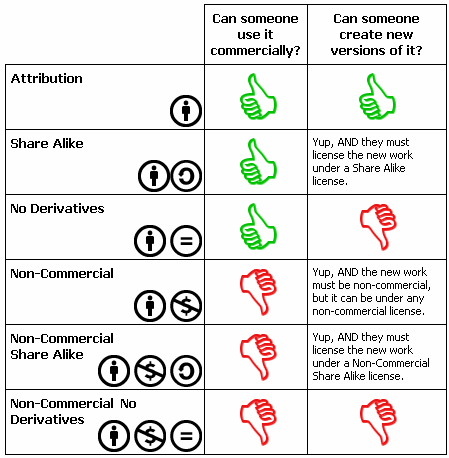
\includegraphics[height=0.7\textheight]{../img/cc-list}

    \begin{large}Copyright (\copyright) \end{large}
  \end{center}
\end{frame}

\begin{frame}
  \frametitle{How to use Creative Commons Licenses}

  Creative Commons has a guide to walk you through the process of generating a license you can attach to your content: \href{http://creativecommons.org/choose/}{creativecommons.org/choose/}

  \begin{center}
    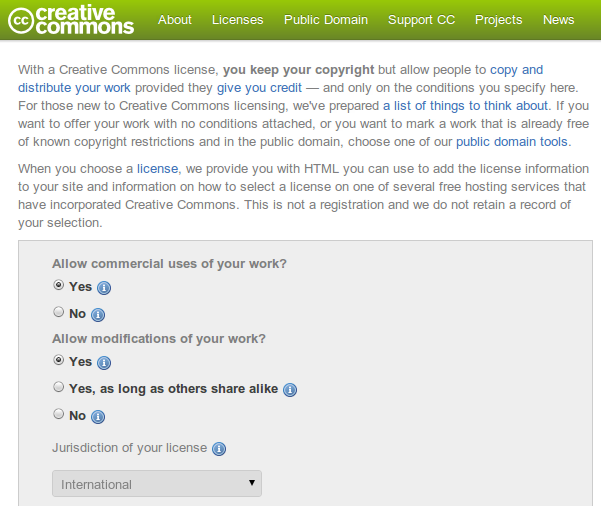
\includegraphics[height=0.7\textheight]{../img/cc-guide-short}
  \end{center}
  
\end{frame}

% http://news.ycombinator.com/item?id=3099362


\begin{frame}
  \begin{center} \begin{Huge}Get it out there!\end{Huge} \end{center}
\end{frame}

\begin{frame}
  \frametitle{Github}
  \begin{center}
    
\includegraphics[width=0.3\textwidth]{../img/octocat}

    
\includegraphics[width=0.3\textwidth]{../img/github-logo}

    github.com

  \end{center}
\end{frame}

\begin{frame}
  \frametitle{Github}
  \begin{center} 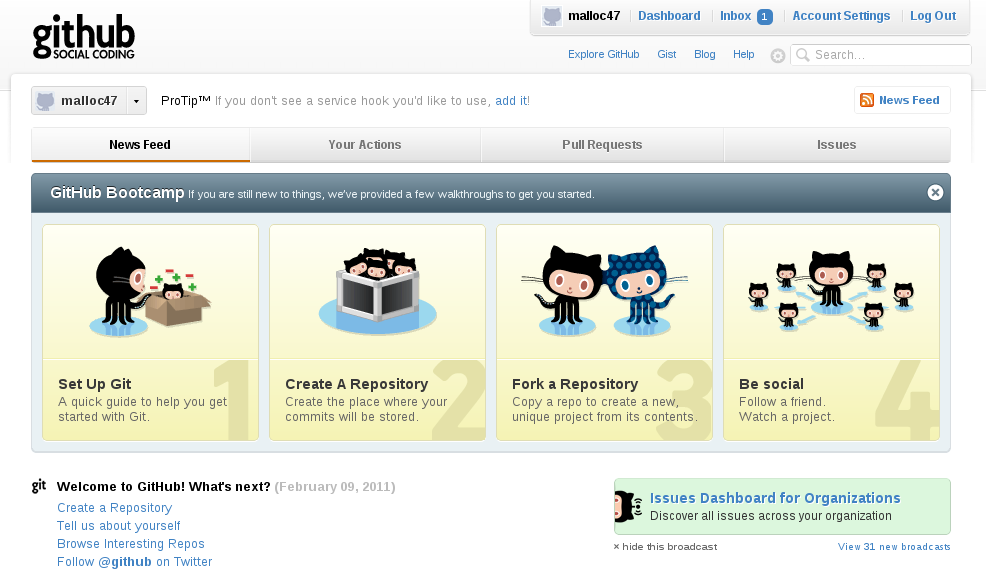
\includegraphics[width=1\textwidth]{../img/github-screenshot} \end{center}
\end{frame}

% \begin{frame}
%   \frametitle{About Github...}
%     \begin{Large}
%       When it comes to hiring, I'll take a Github commit log over a
%       resume any day.
%       \begin{flushright}
%         \textemdash{}John Resig
%       \end{flushright}
%   \begin{center} 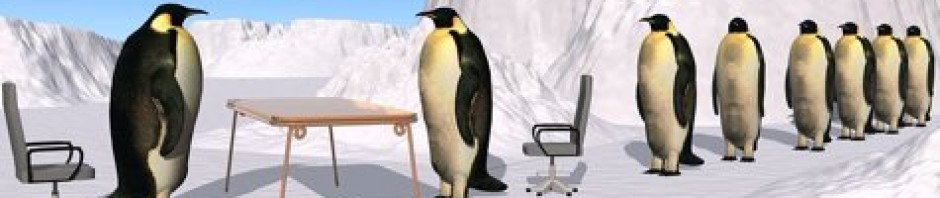
\includegraphics[width=0.5\textwidth]{../img/tux-interview} \end{center}
%     \end{Large}
% \end{frame}

% \begin{frame}
%   \frametitle{How?}
%   \begin{itemize}
%     \setlength{\itemsep}{2em}
%   \item \begin{LARGE} Contribute \end{LARGE} \\ (to existing projects)
%   \item \begin{LARGE} Create \end{LARGE} \\ (your own projects and make them open source)
%   \end{itemize}
% \end{frame}

% \begin{frame}
%   \begin{center}
%     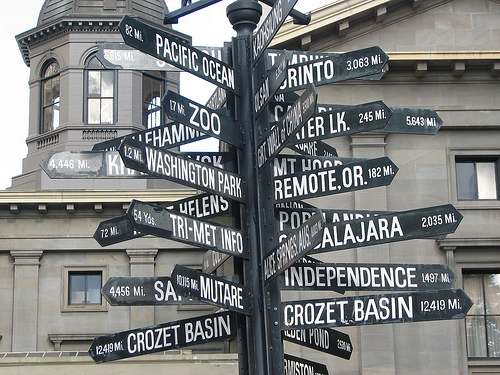
\includegraphics[width=0.75\textwidth]{../img/road-sign}

%     Know the territory...
%   \end{center}
% \end{frame}

% \begin{frame}
%   \begin{center}
%     
\includegraphics[width=0.75\textwidth]{../img/cat-expert}

%     ...if you want to be an expert
%   \end{center}
% \end{frame}

\begin{frame}
  \frametitle{Stuff you may need (might not be taught in school!)}
  % \begin{overlayarea}{\textwidth}{\textheight}
    \begin{itemize}
    \item Language: whatever the project is written in
    \item Build Process: Make, CMake autotools, Ant, Jam, Rake
    \item Version control: git, CVS, svn, Bazaar, Darcs, Mercurial
    \item Bug Trackers: Bugzilla, Trac, Mantis, Launchpad
    \item Communication: Forums, Wikis, IRC
    \item Source Code Communities: github, Bitbucket, Launchpad,
      Gitorious, Google Code, SourceForge
    \item Play nice in other people's sandbox!
    \end{itemize}
  % \end{overlayarea}
    
    \begin{center}
      You may not learn it all in school!
    \end{center}
\end{frame}

\begin{frame}
  \frametitle{The Short Answer}
  \begin{center}
    \begin{Large}
      \textcolor{beamer@myblue}{Contribute} or \textcolor{beamer@myblue}{create}, do \textcolor{beamer@mygreen}{documentation} or \textcolor{beamer@mygreen}{development}, \textcolor{beamer@mygrey}{share} whatever you do wherever you go, but just
    \end{Large}

    \vspace{3em}

    \begin{Huge}
      Get Involved!*
    \end{Huge}
  \end{center}

\vspace{7em}

\begin{footnotesize}
  *Minimal pressure
\end{footnotesize}

\end{frame}

\begin{frame}
  \begin{center}
    \begin{Huge}Summary\end{Huge}
  \end{center}
\end{frame}

\begin{frame}
  \frametitle{What you need to remember from today}
  \begin{center}
    \begin{Huge}
      Open Source $\Rightarrow$ Opportunity

      \vspace{1em}

      Open Source $\Rightarrow$ Employment

      \vspace{1em}
      
      Open Source $\Rightarrow$ Involvement
    \end{Huge}
  \end{center}
\end{frame}

% http://www.kegel.com/academy/opensource.html
% http://stackoverflow.com/questions/43649/how-to-get-involved-in-an-open-source-project

\end{document}
